\documentclass[a4paper,12pt]{article}
%\documentclass[a4paper,10pt]{scrartcl}

\usepackage[margin=0.95in]{geometry}
\usepackage[utf8]{inputenc}
\usepackage{graphicx}
%\documentclass{minimal}
\usepackage{amsmath}
\usepackage{xcolor}
\usepackage{listings}
\lstset{
    frame=single,
    breaklines=true,
    postbreak=\raisebox{0ex}[0ex][0ex]{\ensuremath{\color{red}\hookrightarrow\space}}
}
\lstdefinelanguage{numpy}{
    keywords = {mean}
}

\title{Parameter Estimation with Maximum Likelihood Fitting}
\author{B098688}
\date{\today}



\begin{document}
\maketitle

\begin{abstract}
 This report outlines a proposed procedure for using the Maximum Likelihood Fitting method to estimate parameters in a radioactive decay situation. The input for this exercise are from experimental results that document the decay times of some radioactive substance comprised of two components. Using Maximum Likelihood estimations (and Negative Log-Likelihood (NLL) as an appropriate surrogate for it~\cite{erdogan1999monotonic}) it is possible to estimate the fraction of the first component $f$ in the substance, the lifetime of the first component $\tau_1$ and that of the second $\tau_2$. These are found to be $f=0.749 \pm 0.008$, $\tau_1=0.198 \pm 0.002 [s]$, and $\tau_2=1.307 \pm 0.026 [s]$. An error is obtained from these results by looking at values of the NLL by varying each of the three parameters and keeping the other two constant. Finally, a Monte Carlo simulation is created and its errors are compared to those previously obtained. 
\end{abstract}

\section{Introduction}

An important development in statistics during the early $20^{th}$ century was the method of Maximum Likelihood Estimation (MLE). This method attempts to estimate a set of parameters of some statistical model by obtaining the parameter(s) that maximise the likelihood of reproducing observations given said parameter(s)~\cite{aldrich1997ra}. 

In order to perform a MLE it is necessary to have two things: (i) a sample of independent observations and (ii) a probability density function with some (at least one) unknown parameter. The first is given as a datafile named ``DecayTimesData.txt'', and the former is the probability density function of the decay of a radioactive substance composed of two components (each with a characteristic lifetime). This means that the input data is a set of measurements of the decay time of the radioactive substance, and the associated probability density function with three parameters attempts to model such behaviour. What is required is to determine what are the values of these parameters.

Figure~\ref{fig.1} shows a histogram of the input data, where an exponential decay is clearly appreciated. This is characteristic of every radioactive decay, as it is common knowledge that a single particle radioactive decay is directly proportional to $exp(-t/\tau)$, where $\tau$ is the lifetime of the radioactive particle. To go from this behavioural description to a probability density function (PDF) a normalisation constant is introduced. This normalisation constant is such that when the PDF is integrated in time from $0$ to $\infty$, the resulting value is $1$. The physical interpretation of this is that a radioactive particle will definitely decay at some point in time. 

\begin{figure}[h!]
\centering
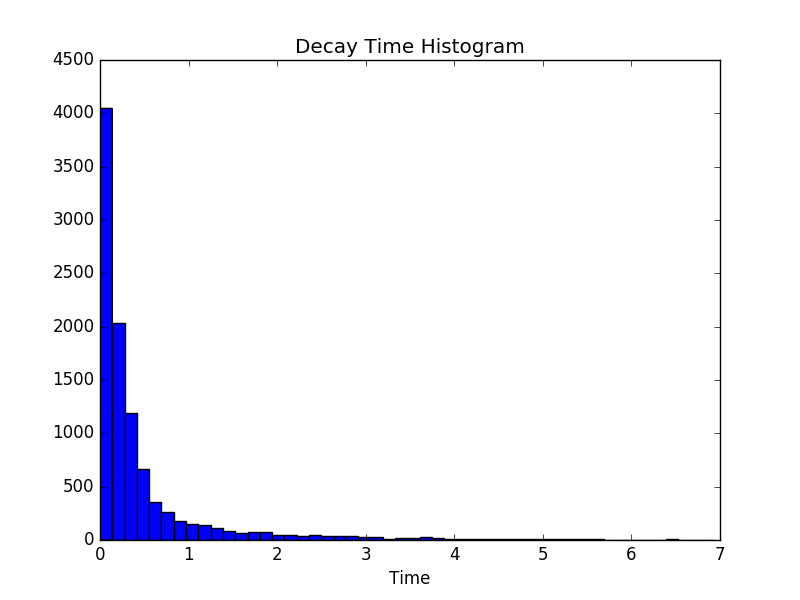
\includegraphics[width=0.75\textwidth]{img/observed_time}
\caption{Observed decay time of the radioactive body.}
\label{fig.1}
\end{figure}

For a radioactive substance composed of two radioactive components, it is possible to describe its decay with an appropriate combination of PDF's of each radioactive component. This can be written as eqn.~\ref{eq.1}, where $f$ is the fraction of the first component in the overall radioactive substance, $\tau_1$ is the lifetime of the first component, and $\tau_2$ is the lifetime of the second component. 

\begin{equation}
 P(t \vert f, \tau_1, \tau_2) = \frac{f}{\tau_1} e^{-t / \tau_1} + \frac{1-f}{\tau_2} e^{-t / \tau_2}
 \label{eq.1}
\end{equation}

Using a minimising algorithm built-in \texttt{scipy.optimise}, a code written in Python3.5 is devised to obtain the parameters that fit eqn.~\ref{eq.1} to the observed decay data (``DecayTimesData.txt''). These parameters are found to be  $f=0.749 \pm 0.008$, $\tau_1=0.198 \pm 0.002 [s]$, and $\tau_2=1.307 \pm 0.026 [s]$. In order to analysing the input data, the \texttt{numpy} library is used, and \texttt{matplotlib.pyplot} to plot the results. Some comments are given regarding how these errors were obtained. 

Finally, $500$ Monte Carlo simulations are performed, each with $10000$ decay times, and the minimising parameters of each simulation is obtained to compare the errors. An average of these Monte Carlo parameters is taken and are $f=0.740 \pm 0.010$, $\tau_1=0.196 \pm 0.019 [s]$, and $\tau_2=1.239 \pm 0.054 [s]$. In order to obtain the errors for the Monte Carlo simulation careful considerations were made. Three methods for obtaining the errors for each parameter are considered: the common Jacknife method was, the standard deviation of all Monte Carlo simulation's parameters and the traditional $1/\sqrt{N_{MC}}$. All these methods have a good concordance among themselves. This will be briefly reviewed later on.

\section{Aim and Methods}

The aim of this problem is to take an input set of observed decay times and use them to obtain the probability density function (PDF) that accurately models such behaviour. To do so, a Maximum Likelihood Estimate (MLE) is used to determine three parameters ($f$, $\tau_1$, and $\tau_2$). This is done by first getting the ``joint likelihood'' function described in eqn.~\ref{eq.2}. Changing the three parameters such that this joint likelihood function is maximised will give the best fit parameters.

\begin{equation}
 \mathcal{L} = \Pi_i P(t_i \vert f, \tau_1, \tau_2)
 \label{eq.2}
\end{equation}

It is also possible to use the Negative Log-Likelihood ($\mathcal{NLL}$), which is computationally more stable since it transforms a sequential multiplication to a logarithmic sum. This is created by eqn.~\ref{eq.3}, and it is implemented in the aforementioned code. This is morphologically similar to the joint likelihood function, but inverted. That means that in order to obtain the best fit parameters a minimisation of the $\mathcal{NLL}$ function is required.

\begin{equation}
 \mathcal{NLL} = -\log \mathcal{L} = - \sum_i \log P(t_i \vert f, \tau_1, \tau_2)
 \label{eq.3}
\end{equation}

The minimisation should take as values the observed decay times (the elements of the input file ``DecayTimesData.txt'') and vary only the three parameters ($f$, $\tau_1$, and $\tau_2$). Note that these should be constrained to be positive, and $f$ between the open interval $(0:1)$ (which is open since the PDF starts assuming that there are two components in the radioactive solution). 

To obtain these parameters the following procedure is used: 

\begin{enumerate}
 \item Create $\mathcal{NLL}(observed\_times,\,parameters)$ function.
 \item Initialise the parameters (init\_params=$(0.01, 0.01, 0.01)$ fulfills all restrictions).
 \item Bound the possible parameters (bound=$((0.01, 0.99), (0.01, None), (0.01, None))$).
 \item Start the minimiser: $scipy.optimize.minimize(\mathcal{NLL},$ init\_params, method=``SLSQP'', args=(observed\_times,), bounds=bound).
\end{enumerate}

\begin{figure}[h!]
\centering
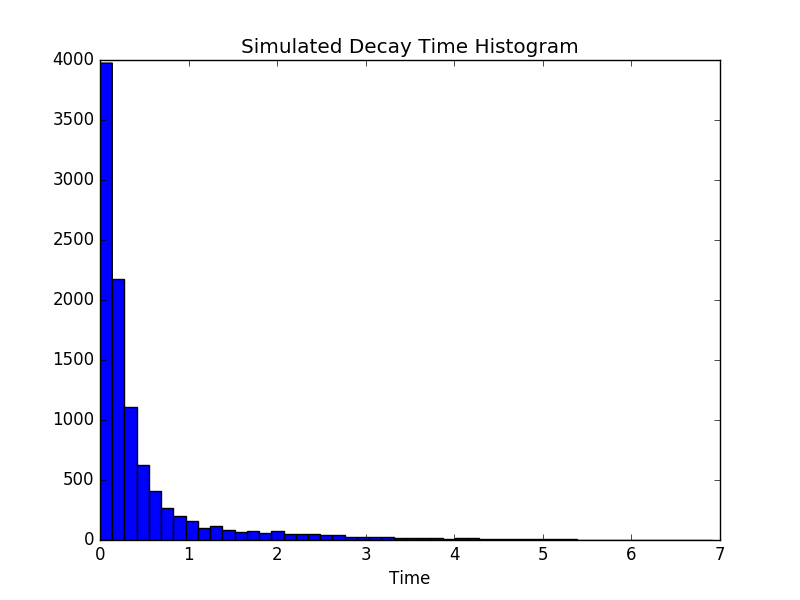
\includegraphics[width=0.75\textwidth]{img/simulated_time}
\caption{Simulated decay time of the radioactive body.}
\label{fig.2}
\end{figure}

The method ``SLSQP'' is used as it supports (unlike other scipy.optimize.minimize methods) imposing bounds on the possible parameters. Among other things, the method returns the parameters that minimise the given function. The ``observed\_times'' input is an array full of the elements in the input data file. Using the obtained parameters, one Monte Carlo simulation is run for $10000$ points. The histogram that sumarises the results from said simulation is shown in fig.~\ref{fig.2}.

A study of the errors obtained from this method can also be obtained. In order to perform a $\chi^2$ error determination it is necessary to vary one parameter about its best fit value (what is obtained from the minimiser by using the observed data) until the value of $\chi^2$ around the minimum is increased by $1$. Similar to this, when using a $\mathcal{NLL}$ minimisation, a $0.5$ increase of the $\mathcal{NLL}$ function when varying one of the three parameters and keeping the other two constant will return the error of the varying parameter. Doing this for all three parameters, their respective error can be obtained. These variations are then plotted. 

Finally, a Monte Carlo series of simulations is generated. By starting with the previously obtained best-fit parameters as input for the probability density function (eqn.~\ref{eq.1}). After setting these parameters, $10000$ decays are simulated by using a random number generator. The simulated decay times are then used to run the minimiser for $\mathcal{NLL}$. This then returns the simulation's best-fit parameters. By running such a simulation $500$ times and saving $f$, $\tau_1$, and $\tau_2$ for each of them, the Monte Carlo simulation is complete. The 500 sets of parameters show a normal distribution, where the mean of each parameter's set of values would be its estimate. The error of each parameter is then calculated by three methods (standard deviation, $1/\sqrt{N_{MC}}$, and Jacknife). The Jacknife method consists of taking each of the $N_{MC}=500$ sets of parameters and removing the $i^{th}$ element, and averaging to obtain $param_i$. This is then compared to the best-fit value of the entire set. The error is then obtained as eqn.~\ref{eq.4}, where $param$ is the average value of the parameter's normal-like distribution. 

\begin{equation}
 \sigma_{Jacknife} = \sqrt{\sum_i^{N_{MC}} (param_i - param)^2}
 \label{eq.4}
\end{equation}

\section{Results and Conclusions}

The first results that are obtained are the observed best-fit parameters originated by using the minimising routine on the observed time data set. These turn out to be the following:

\begin{align}
 f = 0.749 \qquad \qquad \tau_1 = 0.198 [s] \qquad \qquad \tau_2 = 1.307 [s] \nonumber
\end{align}

In order to obtain the errors related to these parameters we follow the process described in the previous section. In doing so, we obtain the following errors:

\begin{align}
 \sigma_f = 0.008 \qquad \qquad \sigma_{\tau_1} = 0.002 [s] \qquad \qquad \sigma_{\tau_2} = 0.054 [s] \nonumber
\end{align}

Then, three plots are created that show the actual value of the $\mathcal{NLL}$ function within a variation of one parameter from its determined value and $\pm3$ times the obtained error while keeping the other two parameters constant and on their observed best-fit values. These are shown in fig.~\ref{fig.3},~\ref{fig.4}, and~\ref{fig.5} for each parameter. 

\begin{figure}[h]
\centering
\begin{minipage}{.32\textwidth}
  \centering
  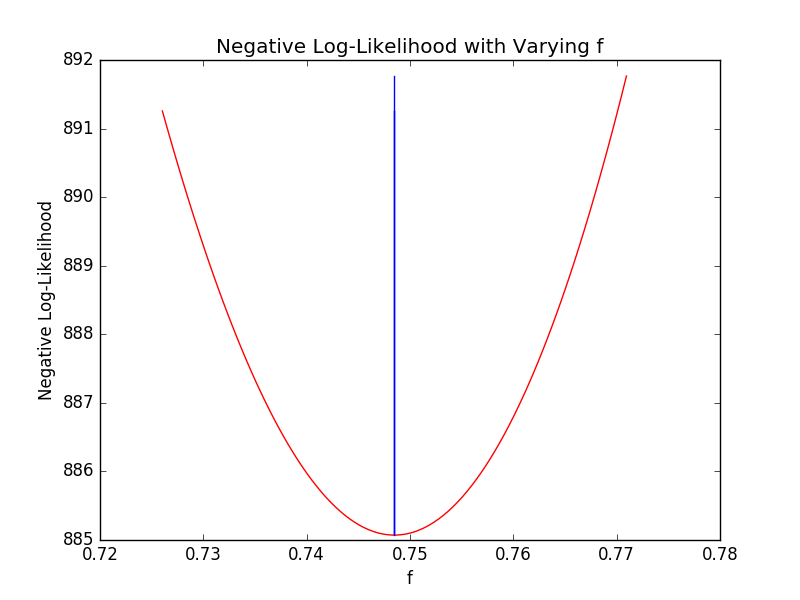
\includegraphics[width=1.05\linewidth]{img/fraction_varyingNLL}
  \caption{$f=0.749$ with $\sigma_f~=~0.008$.}
  \label{fig.3}
\end{minipage}%
\begin{minipage}{.32\textwidth}
  \centering
  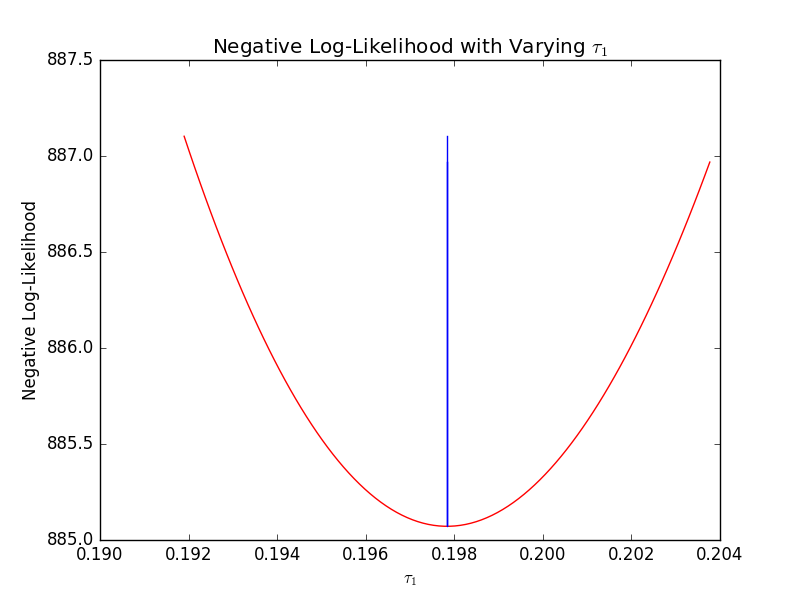
\includegraphics[width=1.05\linewidth]{img/tau1_varyingNLL}
  \caption{$\tau_1=0.198$ with $\sigma_{\tau_1}=0.002$.}
  \label{fig.4}
\end{minipage}
\begin{minipage}{.32\textwidth}
  \centering
  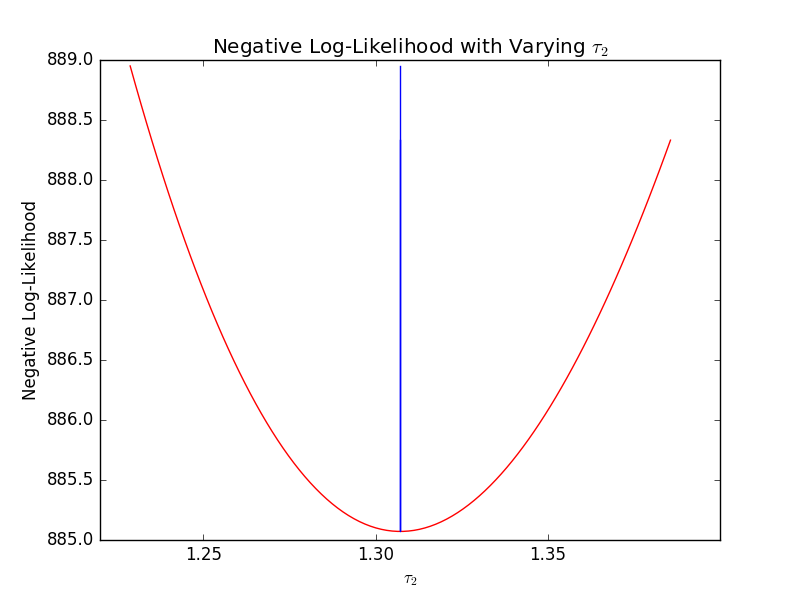
\includegraphics[width=1.05\linewidth]{img/tau2_varyingNLL}
  \caption{$\tau_2=1.307$ with $\sigma_{\tau_2}=0.054$.}
  \label{fig.5}
\end{minipage}
\end{figure}

We now use the observed best-fit parameters to generate Monte Carlo simulations that follow the probability distribution function (eqn.~\ref{eq.1}). First, one simulation with 10000 (the same as the observed times data set) is generated - the histogram that summarises said simulation is the one shown in fig.~\ref{fig.2}. The resemblance between the simulated set and the observed set of decay times is noticeable. However, in order to tell whether the simulated set is a good representation of the observed set a minimisation of the $\mathcal{NLL}$ function has to be performed by using the Monte Carlo simulated data instead of the observed data. 

Doing such an estimation of the parameters for only one simulated data set will not be enough to compare the simulated data set to the observed. In order to properly compare a simulated experiment to a real experiment it is necessary to obtain a statistical sample. To do so, various Monte Carlo simulations (500) that have as input the observed best-fit values ($f = 0.749, \,\tau_1 = 0.198 [s], \,\tau_2 = 1.307 [s]$) are generated and the $\mathcal{NLL}$ function is minimised for each simulation in order to obtain an average of the simulated best-fit parameters.

From this, 500 sets of values of each parameter are obtained. These are then plotted in a histogram (fig.~\ref{fig.6}, fig.~\ref{fig.7}, and fig.~\ref{fig.8}). The mean value of each parameter is also calculated, and found to be:

\begin{align}
 simulated\_f = 0.740 \qquad \qquad simulated\_\tau_1 = 0.196 [s] \qquad \qquad simulated\_\tau_2 = 1.239 [s] \nonumber
\end{align}

\begin{figure}[h]
\centering
\begin{minipage}{.32\textwidth}
  \centering
  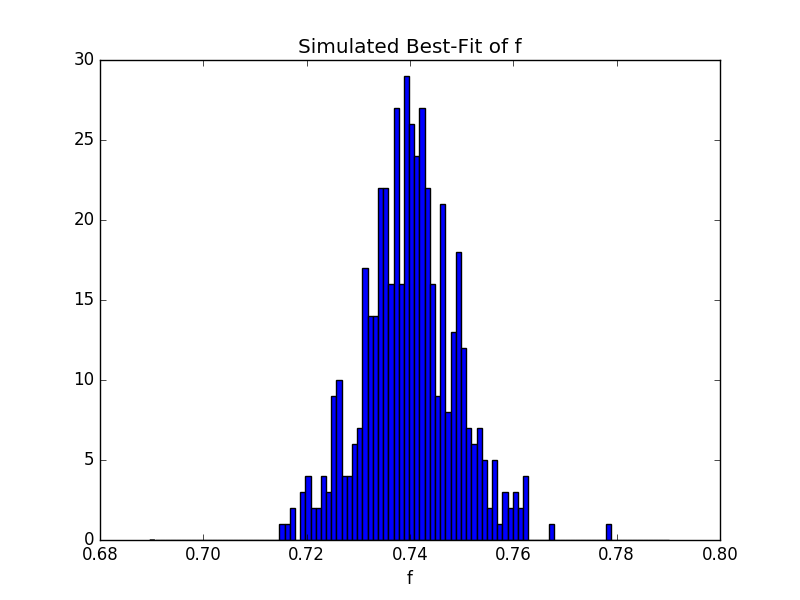
\includegraphics[width=1.05\linewidth]{img/simulated_f}
  \caption{Simulated $f$.}
  \label{fig.6}
\end{minipage}%
\begin{minipage}{.32\textwidth}
  \centering
  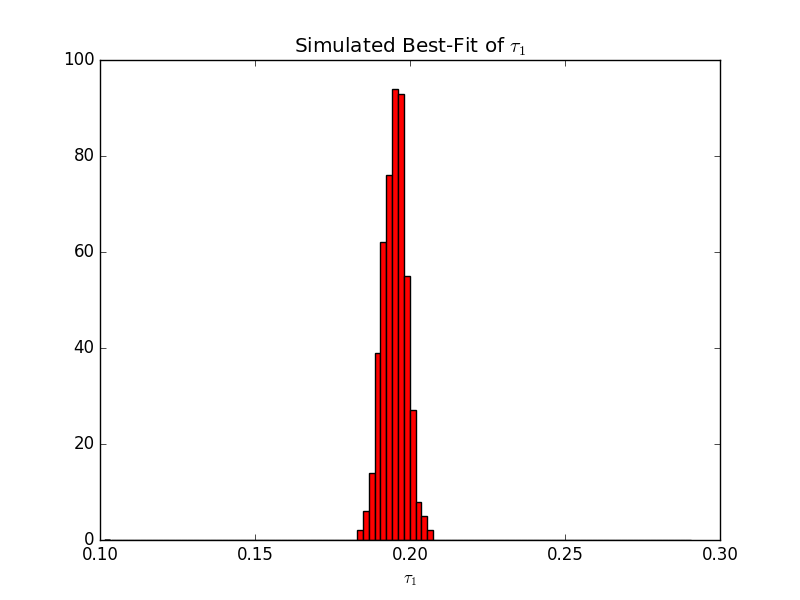
\includegraphics[width=1.05\linewidth]{img/simulated_tau1}
  \caption{Simulated $\tau_1$.}
  \label{fig.7}
\end{minipage}
\begin{minipage}{.32\textwidth}
  \centering
  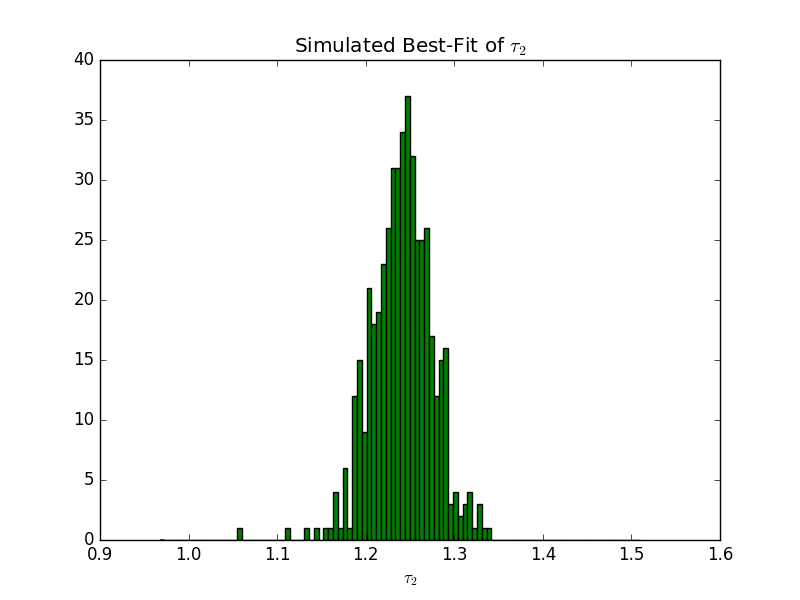
\includegraphics[width=1.05\linewidth]{img/simulated_tau2}
  \caption{Simulated $\tau_2$.}
  \label{fig.8}
\end{minipage}
\end{figure}

After getting the mean values of each simulated best-fit parameter, the next thing is to determine the error in the measurements. This is obtained in three different ways, and they are all found to be similar. The first method is the Jacknife, and the errors have a similar trend to that of the observed best-fit parameters, and they are: 

\begin{align}
 \sigma_{Jacknife\_f} = 0.004 \qquad \qquad \sigma_{Jacknife\_\tau_2} = 0.008 [s] \qquad \qquad \sigma_{Jacknife\_\tau_2} = 0.014 [s] \nonumber
\end{align}

The second method was to obtain the standard deviation of each of the simulated best-fit parameters. This can be done with \texttt{numpy}'s built in routine. For 500 Monte Carlo simulations, the values obtained are:

\begin{align}
 \sigma_{f} = 0.010 \qquad \qquad \sigma_{\tau_2} = 0.019 [s] \qquad \qquad \sigma_{\tau_2} = 0.054 [s] \nonumber
\end{align}

The last method for calculating the error of the Monte Carlo simulation is to simply get the inverse square root of the number of Monte Carlo simulations performed. This is $\sigma = 1 / \sqrt{N_{MC}} = 0.045$. 

Taking each simulated best-fit parameter it is clear that all of them are inside the observed -best-fit parameter's error (or extremely close). 

\subsection{Conclusions}

After obtaining a set of experimental data of the decay time of a radioactive substance comprised of two components, each with their characteristic lifetimes, a Maximum Likelihood Estimation method was used in order to obtain what we call ``observed best-fit parameters''. These were determined to be $f=0.749 \pm 0.008$, $\tau_1=0.198 \pm 0.002 [s]$, and $\tau_2=1.307 \pm 0.026 [s]$, where $f$ is the fraction of the component with lifetime $\tau_1$.The method used was focused on minimising the Negative Log-Likelihood function of the probability distribution function (PDF) of eqn.~\ref{eq.1}, that is defined by eqn.~\ref{eq.3}. This was done with the \texttt{scipy.optimise} library.

After determining these values, a series of Monte Carlo simulations that followed the PDF of eqn.~\ref{eq.1} were created. For each of these simulations, 10000 decay times were found and then the ``simulated best-fit parameters'' was found for each simulation by using the same method that was implemented for the observed times. Averaging out all the ``simulated best-fit parameters'' for 500 Monte Carlo simulations, the obtained parameters were $f=0.740 \pm 0.010$, $\tau_1=0.196 \pm 0.019 [s]$, and $\tau_2=1.239 \pm 0.054 [s]$. These are all within the error margins of the ``observed best-fit parameters''. However, they are not exactly the same, so we can say that the Monte Carlo simulation results are biased. This bias is $0.009$ for $f$, $0.002$ for $\tau_1$, and $0.0.68$ for $\tau_2$. 

\newpage

\appendix

\section{Algorithm}

The algorithm used to synchronise the input images is divided into two Python files. The first declares an \texttt{Image} class with the required functions to fix the input image, and the second calls for the user to state what they want image they want to input, and whether or not they want to save the output image. 

\subsection{\texttt{Image.py}}

\begin{lstlisting}[language=numpy]
import numpy as np
import matplotlib.pyplot as plt
from scipy import misc
import os


class Image(object):
    """
     Class to fix a .pgm image with randomly shifted lines.
    :param fileName is the path to a .pgm file
    """

    image = 0.
    cols = 0
    rows = 0

    threshold_top = 0.995 # Maximum value of normalised cross correlation to consider shifting.
    threshold_bottom = 0.8 # Minimum value of normalised cross correlation to consider shifting.

    def __init__(self, fileName):

        self.fileName = str(fileName)
        self.image = misc.imread(self.fileName)
        self.cols = len(self.image)
        self.rows = len(self.image[0])

    def get_xcorrelation(self, line_number):
        """
        :param line_number: int from 1 to rows
        :return: real part of cross correlation between line #line_number and line #line_number-1
        """

        base_line = np.fft.fft(self.image[line_number])
        base_line[:] = (base_line[:]-np.average(base_line))/(np.std(base_line))
        compared_line = np.fft.fft(np.roll(self.image, 1, axis=0)[line_number])
        compared_line[:] = (compared_line[:] - np.average(compared_line)) / (np.std(compared_line))
        xcorrelation = np.fft.ifft(np.multiply(base_line, np.conjugate(compared_line)))

        return xcorrelation.real

    def shift(self):
        """
        Use get_xcorrelation() function to shift the input image into place.
        """

        xcorrelation_max = np.zeros(self.cols)
        shift = np.zeros(self.cols, dtype=int)

        for i in range(1, self.cols):

            xcorrelation = self.get_xcorrelation(i)
            shift[i] = (int)(np.argmax(xcorrelation))
            xcorrelation_max[i] = xcorrelation[shift[i]]

            if (shift[i]!=0) & (shift[i] != shift[i - 1]) & \
                    (xcorrelation_max[i] < self.threshold_top) & (xcorrelation_max[i] > self.threshold_bottom):
                """
                If the shift is non zero, and different from the previous shift (to avoid bulk shifting),
                there will be a shift provided the cross correlation maximum is within an appropriate range.
                """
                self.image[i] = np.roll(self.image[i], -shift[i])

    def clean_up(self):
        """
        Proposed function for cleaning up edges.
        Not used
        """
        cleaned_lines = 0
        xcorrelation_argmax = np.zeros(self.rows)

        for i1 in range(1, self.cols-1):

            xcorrelation_argmax[i1] = np.argmax(self.get_xcorrelation(i1)).astype(int)

        for i1 in range(1, self.cols-1):

            if (xcorrelation_argmax[i1] != 0):

                self.image[i1] = np.roll(self.image, 1, axis=0)[i1]
                cleaned_lines += 1

    def show_image(self):

        plt.imshow(self.image, cmap=plt.cm.gray)
        plt.show(block=False)

    def save_image(self):

        if os.path.isdir("img_out") == False:
            os.mkdir("img_out")

        out_image = str("img_out/" + input("Output image name (just name, not the path) : "))
        misc.imsave(out_image, self.image)
\end{lstlisting}

\subsection{\texttt{FixThem.py}}

\begin{lstlisting}[language=numpy]
from Image import *

fn = str(input("Input image name: "))

while(os.path.isfile(fn) == False):

    fn = str("img_in/" + fn)
    try:
        im = Image(fn)
    except IOError:
        print("File does not exist.")
        fn = str(input("Input image name: "))


im = Image(fn)
im.shift()
#im.clean_up()
im.show_image()

ask_save = str(input("Want to save image? (y/n): "))

if(ask_save == "yes" or ask_save == "y"):

    im.save_image()
\end{lstlisting}

\newpage

\bibliographystyle{unsrt}
\bibliography{report2}

\end{document}
